\section{System Overview}
%\section{System Framework}
\label{sec-system}

\begin{figure}
\centering
\subfigure[{\scriptsize Framework}]{\label{fig:framework}
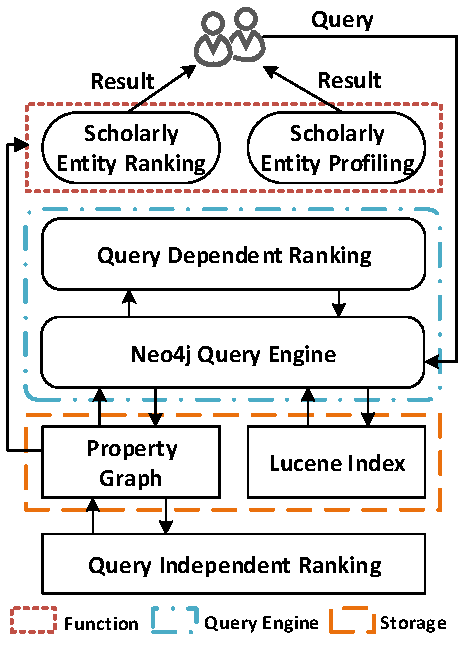
\includegraphics[width=0.4\columnwidth]{systemFrame.pdf}}
\subfigure[{\scriptsize Neo4j schema design}]{\label{fig:schema}
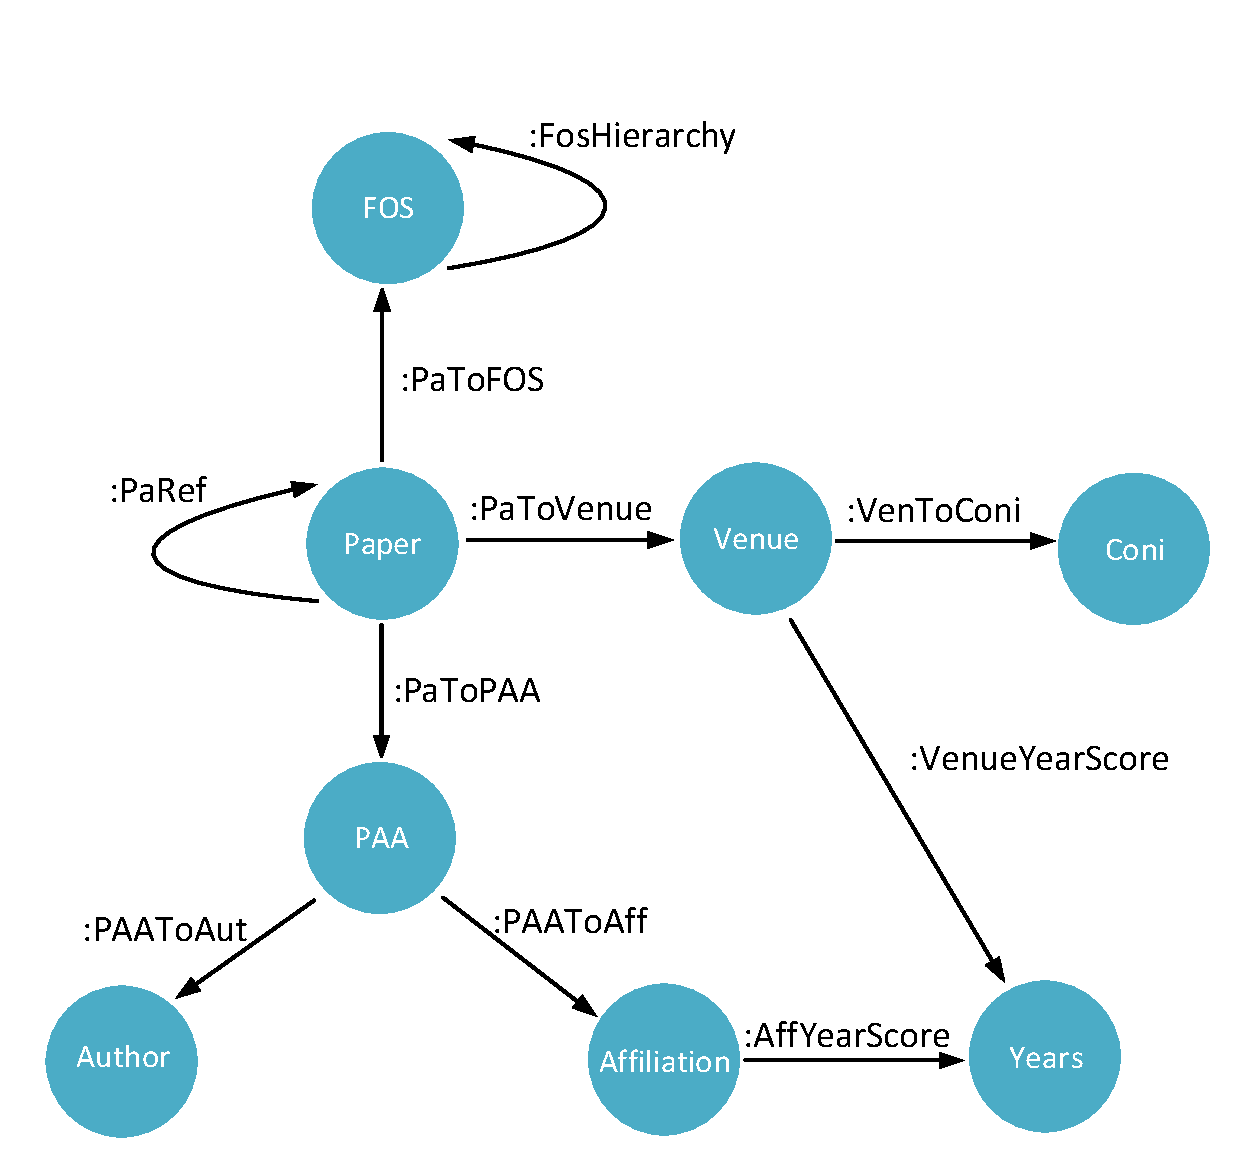
\includegraphics[width=0.4\columnwidth]{neo4jSchema.pdf}}
\caption{System overview of \oursystem}
\label{fig:system}
%\vspace{-2ex}
\end{figure}

\eat{
\begin{figure}
\centering
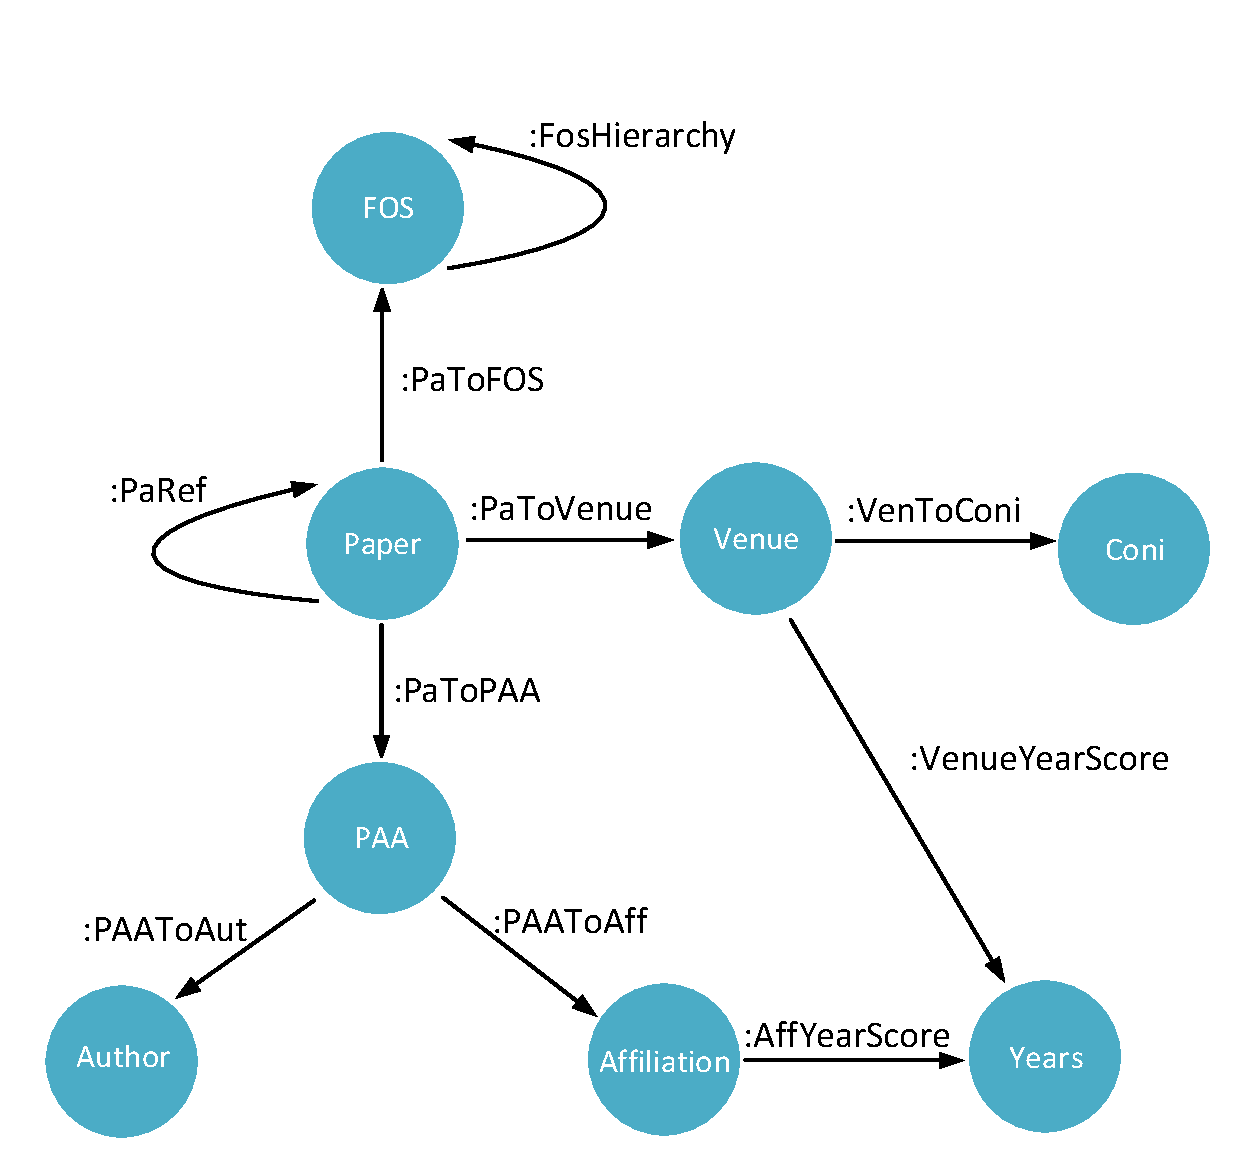
\includegraphics[width=0.5\columnwidth]{neo4jSchema.pdf}
\caption{Neo4j property graph schema design}
\label{fig:schema}
\vspace{-3ex}
\end{figure}
}

(1) Schema design
(2)


Figure \ref{fig:frame} shows the framework of our \oursystem system. It consists of three main components, \emph{Storage}, \emph{Query Engine} and \emph{Visualizer}. We next detail each component.

\marked{highlight graph storage, query engine detail}

\marked{relation to ranking model, when to do ranking}

\marked{incremental computation}
%We mainly use Microsoft Academic Graph(MAG) to build \oursystem ~\cite{sinha2015overview}. It contains about 126 million scientific publication records, 529 million citation relationship and other scholarly activities information. Fig. \ref{fig:frame} shows the framework of our system, which consists of three main components, \emph{Storage, Query Engine} and \emph{Visualizer} respectively. Based on the framework, we then present a set of web-based scenarios using RESTful APIs.
% 126909021 paper  114698044 articles 529 million


%Data source. currently storage solution, shortage, why graph database. storage contents

\subsection{Graph Storage}
%We mainly use Microsoft Academic Graph(MAG) to build \oursystem \cite{sinha2015overview}. It contains scholarly information such as author, article, venue, affiliation, field of study as well as other information. Aminer, CiteSeerx and Semantic Scholar use relational database system such as Mysql to store and manage the xxx.


(1) schema design (reasonale)

(2) property graph (billion-scale) -- lucene index
%(1) adopt neo4j
%(2)

Storage is a key factor for the success of scholarly analysis systems, due to the large volume of scholarly data (\eg \oursystem mainly uses the MAG data with 126 and 529 million articles and citations, respectively~\cite{sinha2015overview}) and the complex entities and relationships.
%
Traditional RDBMS are used by CiteSeerx, AMiner and Semantic Scholar to manage scholarly data. On the other hand, Acemap and Microsoft Academic exploit distributed file systems.
%
We observe that entities in scholarly data are inherently linked. The existing storage solutions all ignore such linked feature, and may face challenges for efficient and high-concurrent query processing when the computing resources are limited. For instance, complex join operations in RDBMS will become the bottleneck when processing queries such as {\em finding all articles of someone's co-authors}.
%
To this end, we propose to utilize a popular graph database Neo4j to store and manage the large-scale, heterogeneous and linked scholarly data in \oursystem.
\marked{RDBMS vs. graph database moved to Introduction}

%Scholarly data highly connected by reference relationship between articles and constructs a huge heterogeneous graph.  Take RDBMS as an example, complex joins and self-joins will incur obviously performance bottleneck when the scholarly dataset becomes more inter-related. A comparison of the performance of querying the cited articles of an article using RDBMS(Mysql) and graph database(Neo4j) is given in table 1. Furthermore, our heterogeneous entities ranking algorithm, a type of Time-Weighted PageRank bases on graph structure, assesses the importance of nodes in a heterogeneous graph. Thus, it utilizes a popular graph database Neo4j to store and manage heterogeneous scholarly data.
% scholarly data source, currently solution, why graph database.

Our storage solution includes the property graph and transactions. The scholarly data is stored as a property graph with nodes and relationships and we use transactions to ensure the predictability of relationship-based queries. \marked{derivatives}
%  which possesses nodes and relationships
In order to efficiently retrieve and rank heterogeneous scholarly entities, we design the Neo4j graph schema following two principles: \marked{(a) nodes for entities and relationships for linked structures (\eg citation, authored-by), and (b) reducing fine-grained relationship names while increase generic relationships qualified with property appropriately}.

%Thus, we model scholarly data as a huge heterogeneous graph, shown in Fig. \ref{fig:schema}, which contains more than one billion nodes and over two billion relationships.
Our property graph schema, shown in Fig. \ref{fig:schema}, contains seven basic types of nodes including paper, author, venue, affiliation, field of study, conference instance (\eg ICDE-2019) and year. In addition, we further introduce an artificial type of nodes, \ie PAA representing paper-author-affiliation tuples, to enhance query efficiency. Finally, the property graph schema also forms a total of ten types of relationships to represent the linked structures between scholarly entities.

%Intuitively, a paper get published in a journal/conference by the author means new edges among paper, author and venue node. By employing ranking model as stated in section \ref{sec-model}, we derive affiliation, author, venue and article ranking score using incremental computation \cite{ma2018query}. And those score is described as a property in the graph schema.
% explain our schema



% design principles and schema.
% We take into consideration of the query ability of the graph schema and adopt specific time and space trade-offs. heterogeneous scholarly entity ranking ?

%In fact, we can apply any other ranking algorithms to rank scholarly entities in the graph schema.

\begin{figure*}[tp]
\centering
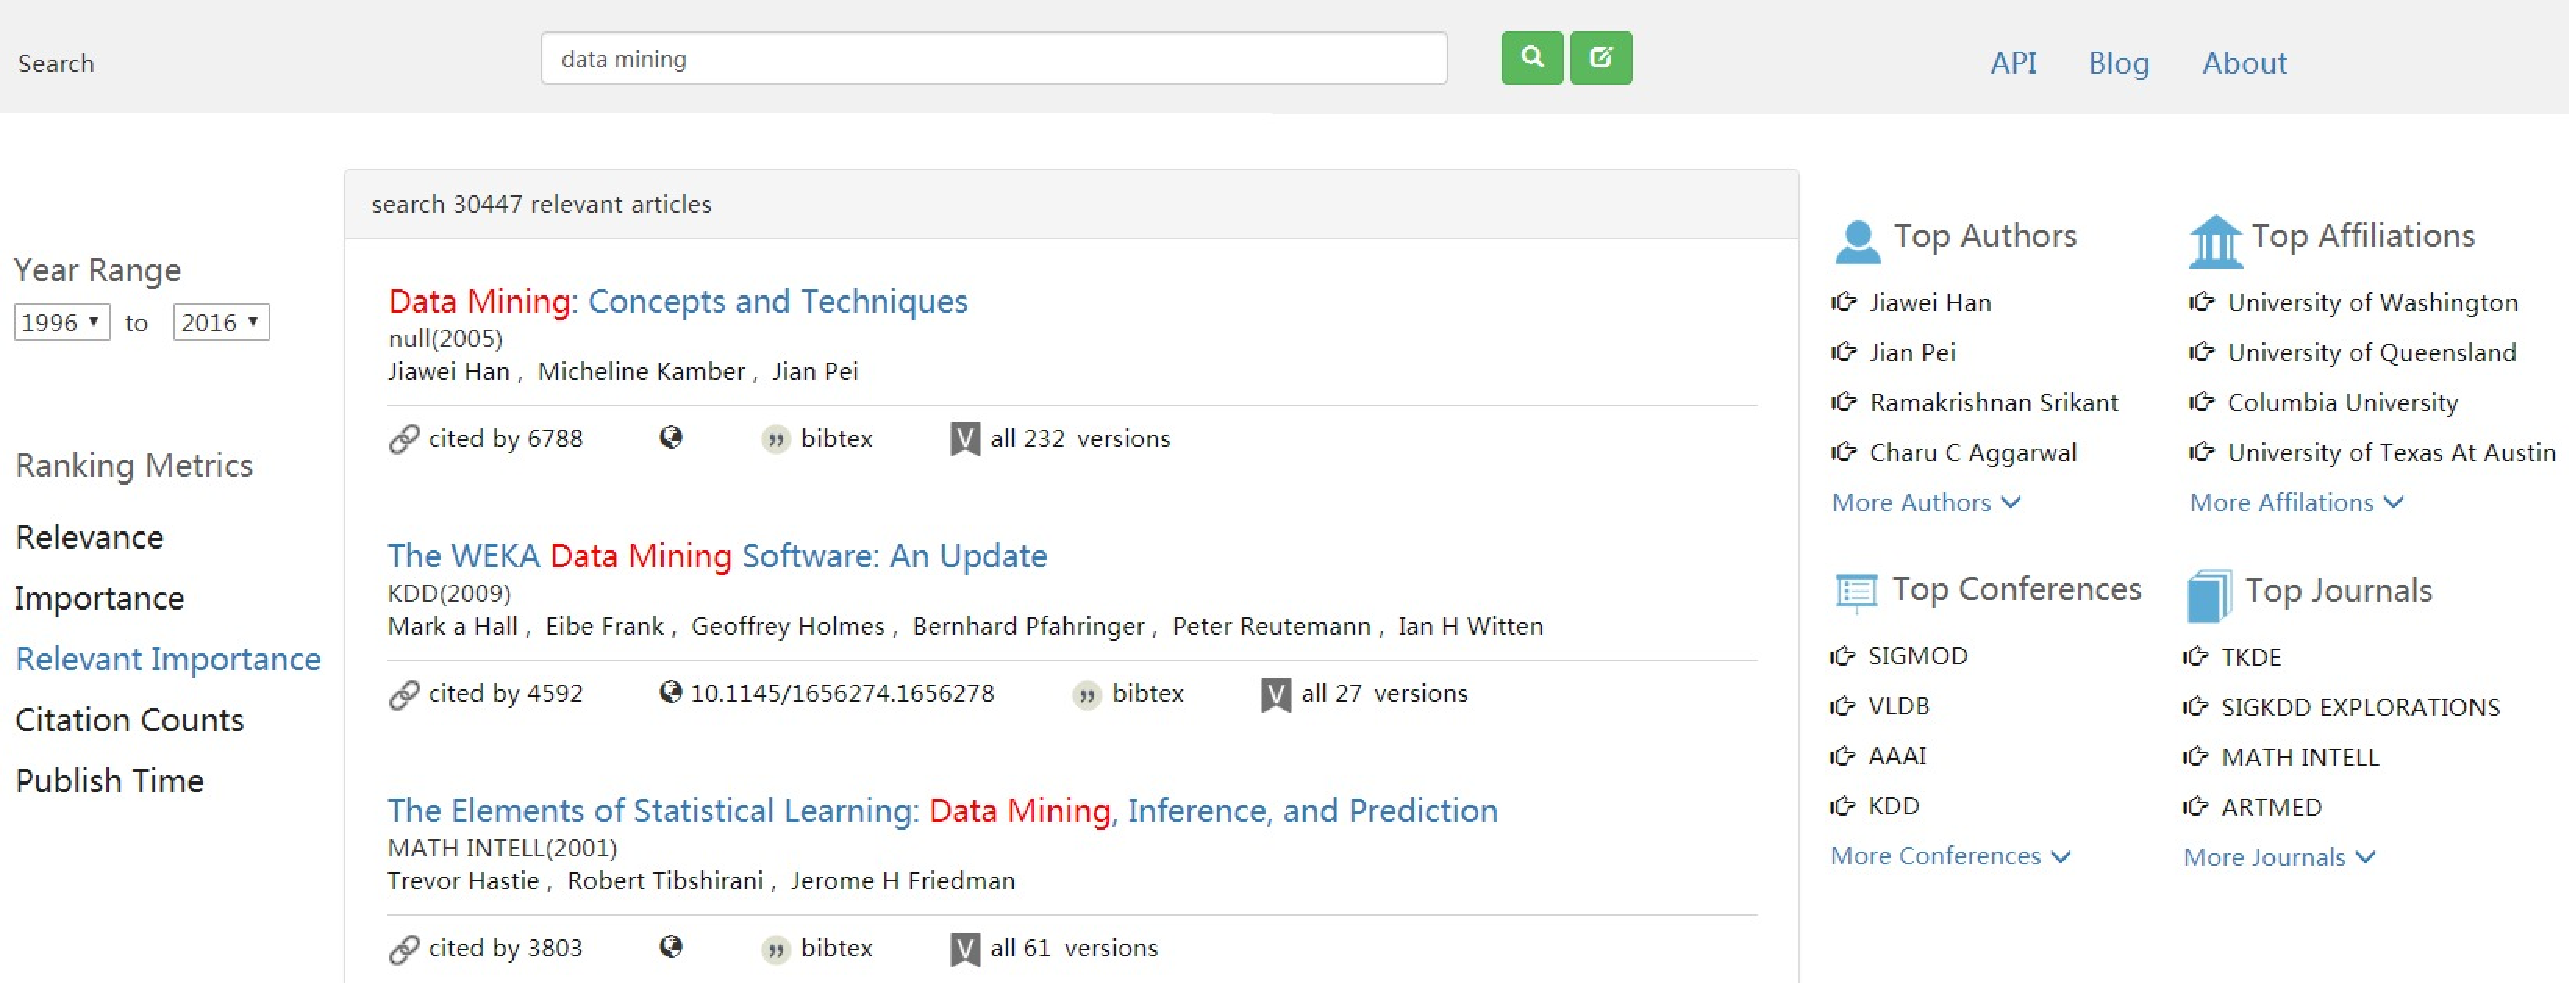
\includegraphics[width=\textwidth]{searchKeywords.pdf}
\caption{Search Keywords And Heterogeneous Entity Ranking}
\label{fig: search keywords}
\vspace{-3ex}
\end{figure*}

\subsection{(Graph) Query Engine}

(1) ranking computation \& incremental
(2) functionality based on query engine
(3) example

\oursystem supports a variety of queries on scholarly data such as keyword retrieval, subgraph search, heterogeneous entity ranking. Query engine is the component responsible for processing a common set of queries on graph database. It consists of the Lucene index, query optimization, Neo4j query engine and ranking algorithms.
% add heterogenous entity Ranking ?

\oursystem takes advantage of Lucene inverted index and \marked{employs Lucene index in property of paper titles, author names and distributed representations of words.
%
Query optimization aims to reduce cardinality of work in the progress to generate a new query plan, such as hitting index, reducing matching paths. Moreover, Neo4j query engine executes the query plan to perform efficient data retrieval.
Finally, search results are aggregated by SARank, relevance, citation, year, average and maximum functions.}


\subsection{Visualizer}
With the development of scholarly data management and processing in the system back-end, the visualizer of \oursystem collects user queries through user interfaces. The queries are dispatched to the query engine and the returned results are then presented by visualizer.
We will demonstrate some scholarly analysis scenarios in the next Section.

\begin{figure}
\centering
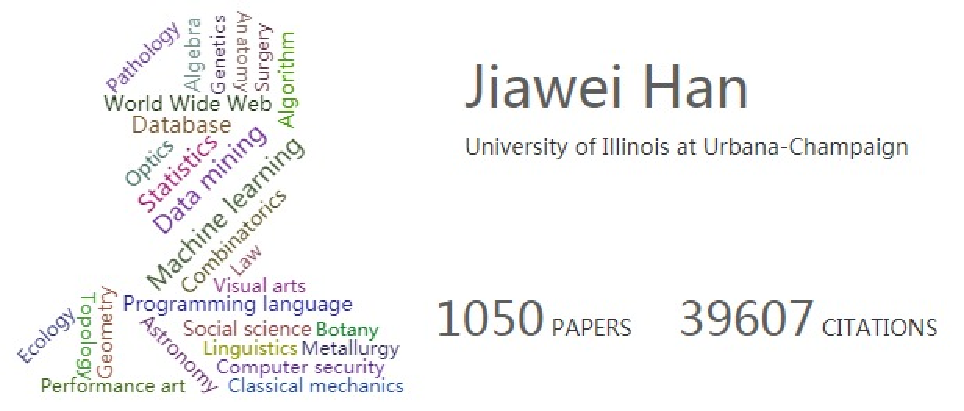
\includegraphics[width=\columnwidth]{hjwAvatar.pdf}
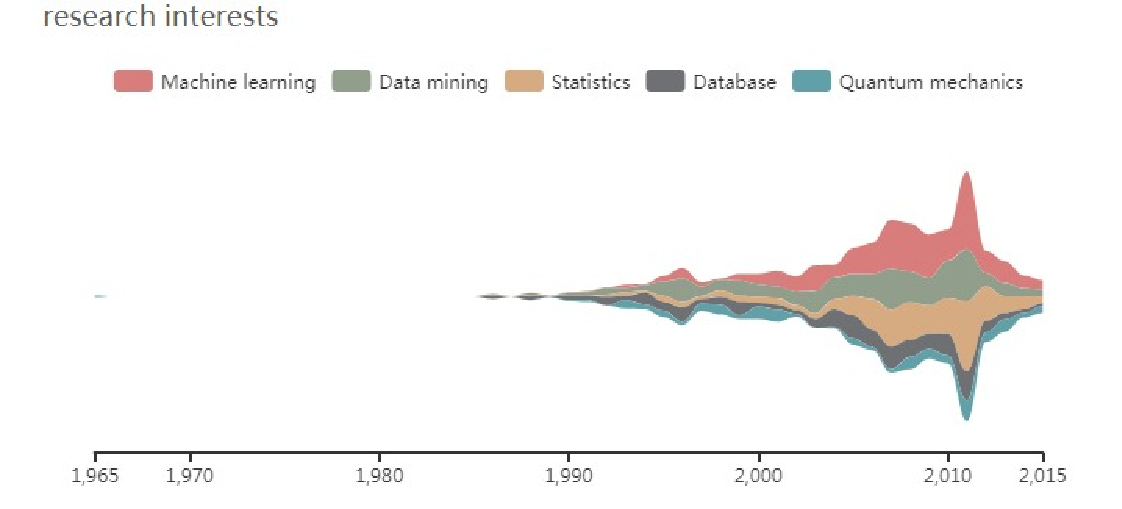
\includegraphics[width=\columnwidth]{hjwInterest.pdf}
%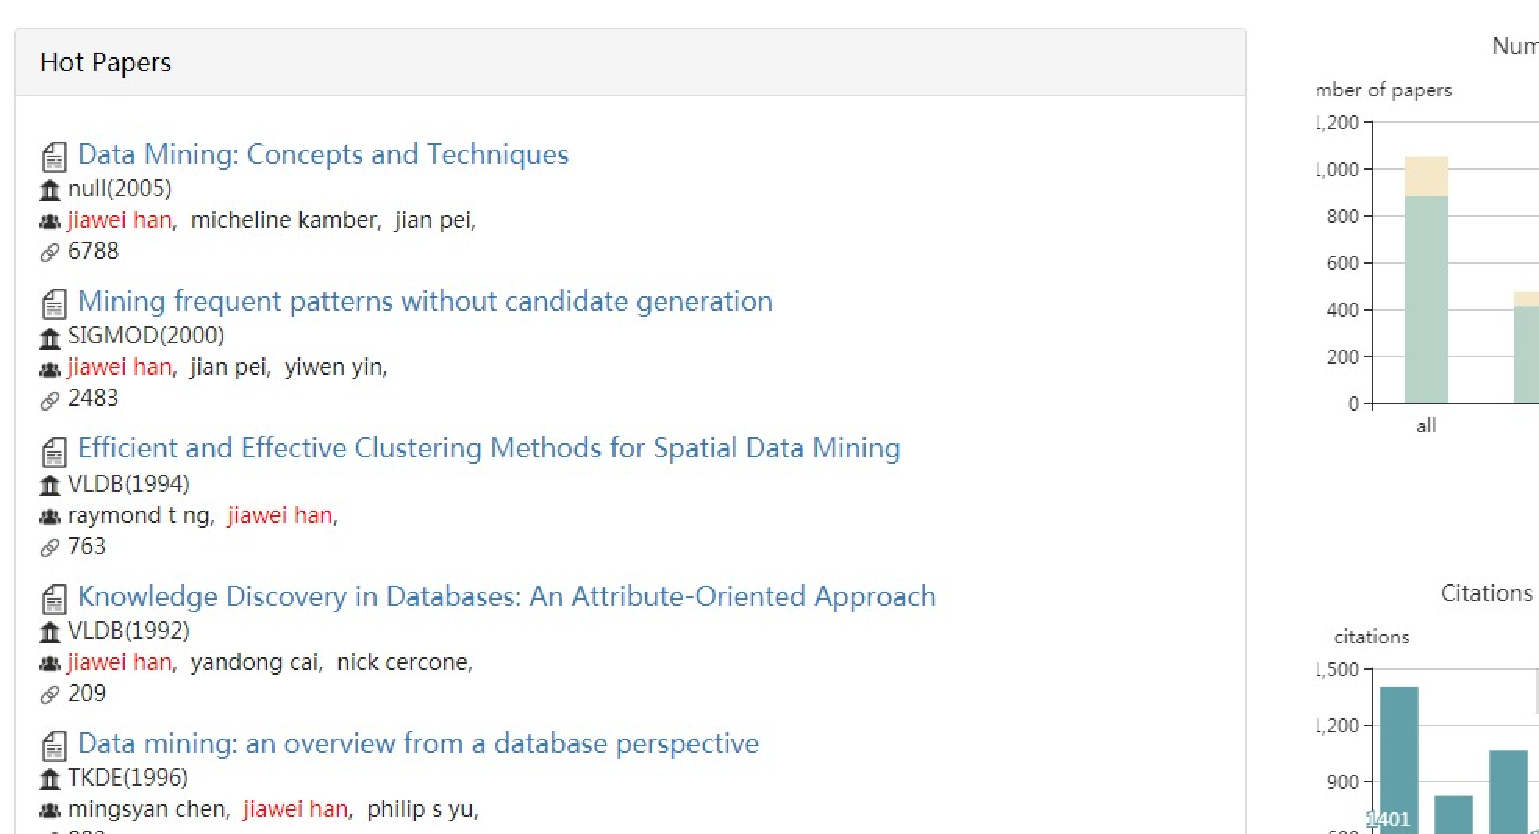
\includegraphics[width=\columnwidth]{hjwPapers.pdf}
\caption{Author Profiling}
\label{fig:hjwProfile}
\vspace{-3ex}
\end{figure}

